\section{Results}

\subsection{360 scan}

When the robot was placed on the center of the arena, it could always find the entrance to the room it wanted to navigate to, no matter its initial orientation.

When the robot was started, during the initial 360 scan, it turned on itself clockwise, using the IR sensors to sense its surroundings.\\
The procedure responsible for the 360 scan waited for both sensors to be higher than a threshold of 180, and identified that as being the only wall that could be perpendicular to the direction the robot was facing. After that, it counted the number of gaps with the left sensor and stopped on the gap of the room of interest.

\begin{figure}[ht]
    \centering
    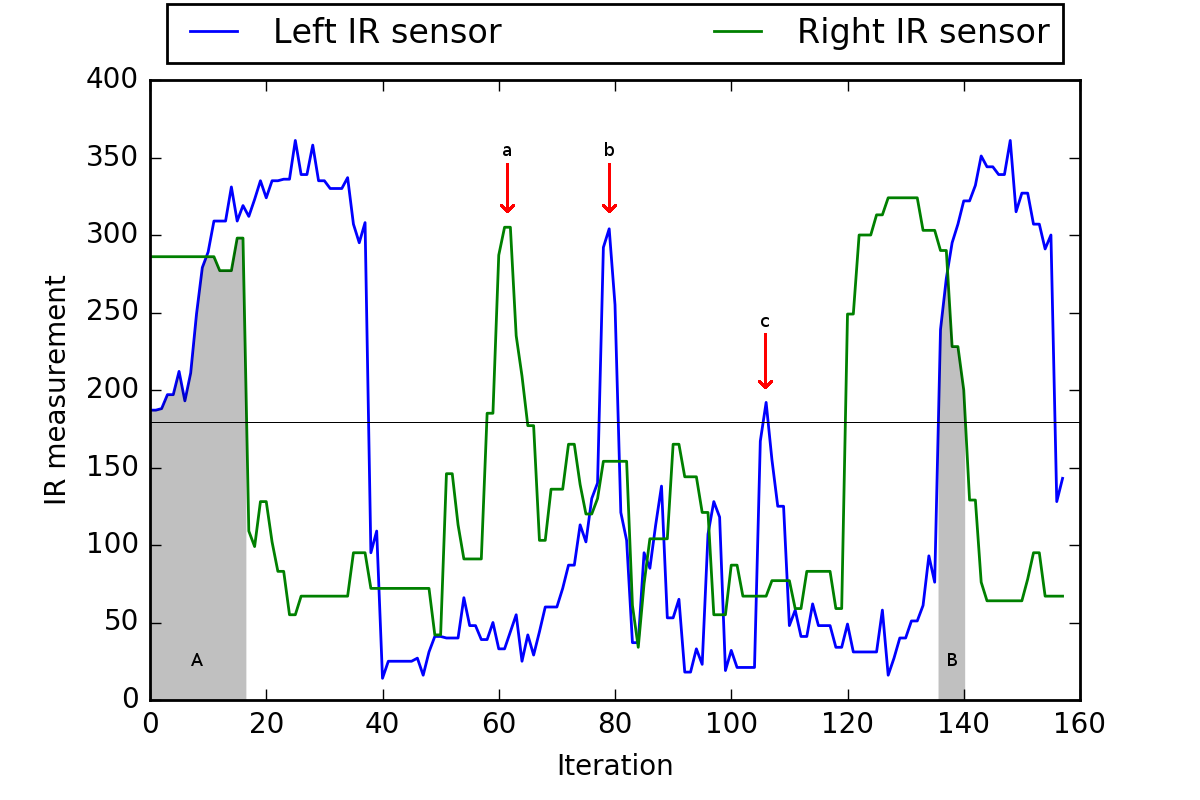
\includegraphics[width=0.7\linewidth]{res/360-scan-plot.png}
    \caption{Samples of the IR sensors while performing a 360 scan at home (the center of the arena). (A) and (B) are the moments when both sensors are triggered past the threshold, i.e., the robot is perpendicularly facing the wall of the center of the arena. (a) and (b) are the moments the right and left sensor pass by the edge of the wall between the entrance for room B and room A, respectively. (c) is when the left sensor passes by the edge of the wall between room A and room C (the smallest of the rooms).}
\end{figure}

% - - - - - - - - - - - - - - - - - - - - - - - - - - -

\subsection{Fetching cube resources}

The robot processed the camera frames by making two copies and cropping each of them: the first would be cropped vertically, removing 2/7 of the width on each side; the second one would be cropped by removing the bottom half of the frame.\\
The first copy would be used to run the Feature Matching (SIFT) algorithm, in order to identify the textures on the resources.\\
The second one would be the long range distance view of the robot, by filtering all colors outside the HSV color space range present in the textures.\\
Cropping these images increased the speed of their post-processing.

The robot was always able to classify the resources at a distance below \SI{0.5}{\m}. It was also always able to identify an object of interest, i.e., a cube resource, up to \SI{1.5}{\m}.

The robot used the coordinates of the contours of the cube on the processed images to calculate its position with respect to the cube. According to that calculation, the robot turned on itself to center the cube resource on its field of view, and then advanced towards the cube 4 hall units.

Occasionally, the cube sensor on the gripper missed the cube, making it believe it did not catch the cube. In such situations, the robot was programmed to back up a little, and re-run the normal procedure.\\
3 out of 10 test runs, the robot had the cube on its gripper but thought it did not. In those cases, the robot backed up and retried to catch the cube.\\
In 1 out of those 3 runs, the robot drifted so much due to the imprecision of its motors that it was not able to get the cube at all.

% - - - - - - - - - - - - - - - - - - - - - - - - - - -

\subsection{Homing after delivering a cube}

The strategy of the robot was to go to the biggest room first, find the cube, deliver the cube to the base on that room, and then return home.\\
To return home, the robot made use of odometry and its sonar to follow the preplanned route from the base to the center of the arena.

Occasionally, when the battery was about to die, the difference in drag between the motors increased, in its turn increasing the drift of the robot as it moved through the arena. Unsurprisingly, in such situation the robot accumulated enough error to not manage to get back home.\\
However, when the conditions were acceptable, i.e., the battery was not dying, and the floor did not have debris, the robot was always able to return home after delivering a cube to the base in room B (the biggest room).

The same did not hold true for homing after delivering a cube to base in room A. The approach used to get the robot back did not work all the times, and needed to be improved for greater reliability.\\
Out of 20 test runs, the robot did not manage to get home in 5 of those runs.\\
Furthermore, since the robot relied on this step to get to the third and last cube, if the robot did manage to return home but did it in a way that it got blocked while doing the last 360 scan, the robot was not able to get the last cube. And this is the reason for the robot to fulfill the complete task very few times.\\
On 9 out of the remaining test runs where the robot managed to get home, it did get stuck.

\newpage
